% !TEX root = demo.tex
\section{Demonstration}
In this section, we detail the proposed demonstration.
The objective of this demonstration is to illustrate 
how \sys enables the rapid iterative construction of data cleaning plans
and the ability to transfer workflows between similar dirty datasets.

\subsection{Datasets}
In our demo, we will consider entity resolution tasks on two different restaurant datasets.
The first dataset contains 858 Zagat reviews\footnote{\scriptsize{ \url{www.cs.utexas.edu/users/ml/riddle/data/restaurant.tar.gz}}},
each tagged with the cuisine of the restaurant reviewed (e.g. ``Chinese" or ``French").
The second dataset is from Yelp and contains 58,127 restaurant records that are also tagged with a category.
In both datasets, tags are inconsistent across records, e.g. ``Chinese" vs. ``Chinese Cuisine".
We will use \sys to merge similar categories together and find the top 10 most popular categories in the dataset.

\begin{figure}[t]
\centering
 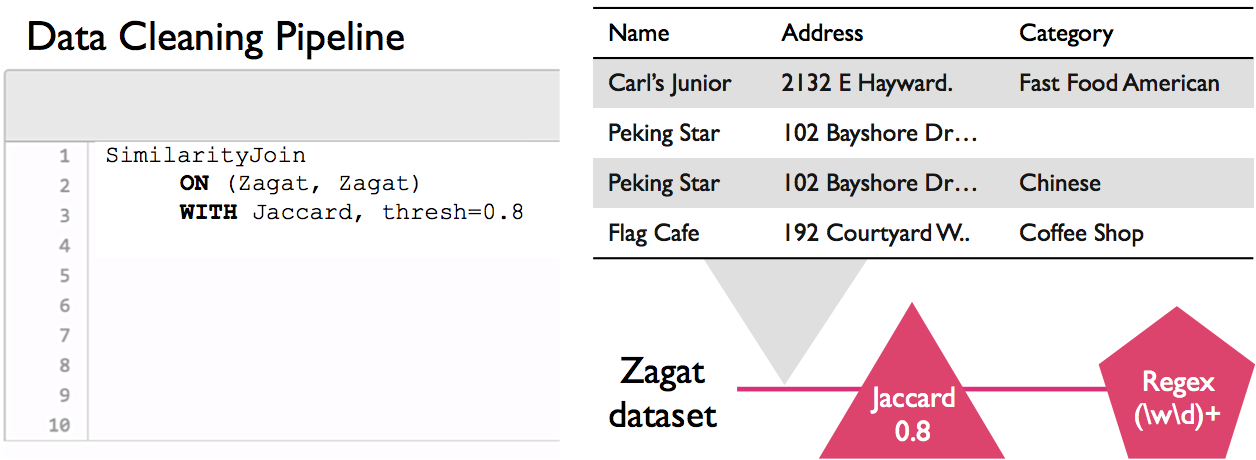
\includegraphics[width=0.75\columnwidth]{figs/dashboard_screenshot.png}
 \caption{The dashboard contains both a visual interface and a text box to specify data cleaning operations. When the user is satisfied, she can run the plan and see the results on the right. \label{screenshot}}
\end{figure}


\begin{figure}[t]
\centering
 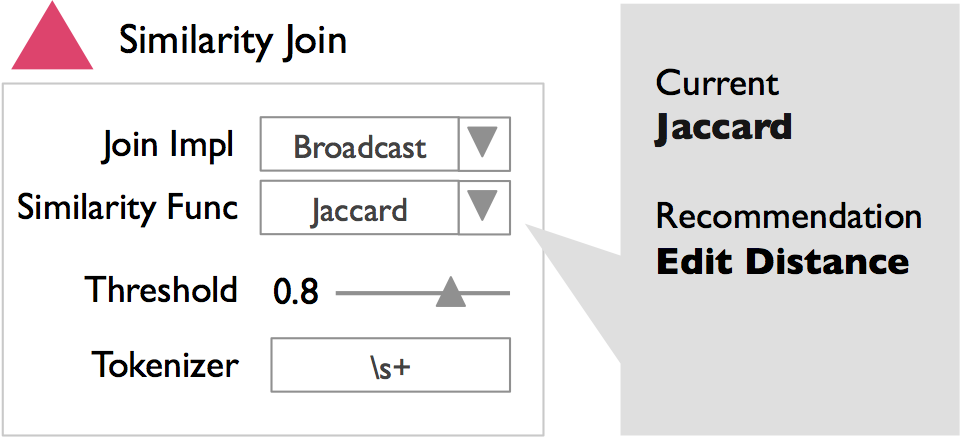
\includegraphics[width=0.65\columnwidth]{figs/dashboard_recsys.png}
 \caption{The operator view lists the parameters of an operator. Users can view recommended changes and modify parameters on the fly.}
 \label{screenshot-rec}\vspace{-1.75em}
\end{figure}

\subsection{Demo Walkthrough}
Now, we will detail the steps of the proposed demonstration.
A screenshot of our dashboard interface is illustrated in Figure \ref{screenshot}.

\vspace{0.2em}

\noindent\textbf{Step 1: } We will explain the components of our dashboard interface to the
demo participants, including how to design data cleaning plans with the visual 
drop down menus, how to compile those plans to our DSL, and how to evaluate the results.

\vspace{0.2em}

\noindent\textbf{Step 2: } Our dashboard will be pre-populated with a data cleaning plan for tag deduplication, and will
start off with the Zagat restaurant dataset. Participants will have the option of choosing one of two Similarity Join implementations, Edit Distance and Jaccard Similarity, and can tune the thresholds for either.
Participants can also add a crowdsourced filtering step in addition to similarity thresholding. 

\vspace{0.2em}

\noindent\textbf{Step 3: } When a participant is satisfied with a plan, they can hit ``Approve" to execute the data cleaning. 
If they chose to use crowdsourcing, then they can complete crowd tasks. 
The results of the plan are visualized in the upper right of our interface.
We show a representative sample of changed records allowing the participant to understand how cleaning affects the data. 
Participants can further analyze their plan by clicking on an operator (Figure \ref{screenshot-rec}).
In addition to the parameters, this shows the recommended changes to the operator.
For example, Figure \ref{screenshot-rec}, shows a recommendation to change the similarity metric from Jaccard to Edit Distance since the attribute in question does not have many tokens.

\vspace{0.2em}

\noindent\textbf{Step 4: } Participants can then switch datasets and observe how the same plan performs on another dataset.
They can modify the plan using the visual interface until the results are satisfactory.
